% Chapter Template
\chapter{Metodologia e Resultados Preliminares}
\label{methods}


%----------------------------------------------------------------------------------------
%	DATA COLLECTION
%----------------------------------------------------------------------------------------

    \section{Coleta de dados}
    \label{collect}

        \subsection{Seleção de hardware}
        \label{hardware}
    
            \paragraph{}
            Para analisar taxa de variação da frequência cardíaca, são necessários sensores de alta precisão, visto que a diferença entre intervalos é da ordem de poucos milissegundos. Existem disponíveis no mercado diversos \textit{smartwacthes} com sensores do tipo PPG (fotopletismografia), mas uma análise prévia da literatura disponível ~\cite{Plews2017ComparisonMethods} revelou que os mesmos não atingem a precisão necessária, especialmente porque geram artefatos de movimento e são sensíveis a diferenças na tonalidade de pele.
            
            \paragraph{}
            Dessa forma, optamos por utilizar um sensor baseado em ECG, que funciona a partir de uma cinta presa no tórax do indivíduo. Esse sensor captura o ECG, executa um pré-processamento para detectar os picos das ondas QRS, e transmite apenas o comprimento dos intervalos RR entre esses picos. Apesar de perder parte da informação contida no ECG completo, essa é uma solução que permite mobilidade e praticidade para o indivíduo, em contraste com uso de eletrodos e aparelhos portáteis de ECG.
            
            \paragraph{}
            Dentre os modelos disponíveis de sensores baseados nessa técnica, optamos por utilizar o H7\textsuperscript{\textregistered}, da fabricante finlandesa Polar. Estudos realizados em laboratório, em conjunto com um exame completo de ECG para comparação, demonstram que esse tipo de sensor apresenta precisão suficiente para capturar a variabilidade ~\cite{Plews2017ComparisonMethods}, e seu custo é relativamente baixo em comparação a outros modelos utilizados em pesquisa. Esse sensor não possui armazenamento interno, porém transmite os dados através de interface \textit{bluetooth low energy}, permitindo sua captura em praticamente qualquer computador ou telefone celular. 

        \subsection{Modelagem do banco de dados}
            
            \paragraph{Volume de dados} Os dados a serem armazenados no banco consistem em uma série temporal com os intervalos RR capturados e uma série de eventos anotados com horário para cada usuário. Para a série de intervalos, estimamos que precisamos de, aproximadamente,
                \begin{equation}
                80 \frac{batimentos}{minuto} \cdot 60 \frac{minutos}{hora} \cdot 24 \frac{horas}{dia} = 115200 \frac{eventos} {dia/individuo}
                \end{equation}
            Se cada evento ocupar um espaço próximo de 32 bytes, teremos em torno de 3.6MB de dados por dia por indivíduo. Para os eventos relacionados às atividades, o volume é consideravelmente menor, por ser registrado em ordem de grandeza de horas. Dessa forma, a série dos batimentos irá dominar o volume ocupado pelo banco de dados.
            
        	\paragraph{}O modelo foi baseado em três tabelas:
            \begin{itemize}
            \item dados do usuário (número identificador, idade, gênero, peso, altura, existência de condições cardíacas, nível de condição física)
            \item intervalos RR (\textit{timestamp}, identificador de fluxo do usuário, valor do intervalo)
            \item registro de atividades (\textit{timestamp} de início, \textit{timestamp} de final, descrição da atividade)
            \end{itemize}
            
            \paragraph{} Os bancos de dados SQL não são otimizados para armazenar séries temporais, por seus índices não serem desenvolvidos para \textit{queries} por intervalos de tempo e também por, de forma geral, não apresentarem escalabilidade suficiente para volumes muito grandes. ~\cite{Dunning2014TimeData} Sendo assim, usaremos um banco de dados NoSQL, adequado para grandes volumes de dados não estruturados.
            
            \paragraph{} Na fase inicial do trabalho, para podermos iniciar a coleta antes de nos preocuparmos com o \textit{setup} do banco, utilizamos um conjunto de arquivos .csv usando o mesmo modelo do banco. É gerado um arquivo por hora para o registro dos intervalos (seguindo um padrão de nomenclatura YYMMDDHH e armazenados em um diretório por indivíduo) e um por dia para o registro das atividades (seguindo um padrão de nomenclatura YYMMDD e no mesmo diretório dos arquivos de intervalo. Os arquivos ficam armazenados no aparelho celular utilizado para coleta e é necessário movê-los para um servidor. Para evitar esse processo, esses dados estão atualmente em processo de migração para um banco de dados NoSQL em tempo real oferecido como serviço em nuvem, o \textit{Google Firestore}. 
        
        
        \subsection{Desenvolvimento de aplicativo}
 	
            \paragraph{} Para realizar a coleta e popular o banco de dados descrito, desenvolvemos um aplicativo móvel, que permite que o registro de intervalos seja realizado automaticamente, de maneira contínua e transparente para o indivíduo, desde que o mesmo esteja utilizando a cinta com o sensor. O aplicativo permite também que o usuário registre manualmente as atividades que estiver executando, como um diário, para treinamento do classificador supervisionado, ou outras variáveis que se deseje controlar em análises futuras.
        
            %%JUINCLUDEFIGURE esquema do aplicativo com sensor e bluetooth
        
            \paragraph{} Isso foi alcançado usando o conceito de serviço foreground, em que um aplicativo garante maior prioridade e menor probabilidade de ser removido da memória ao deixar uma notificação na barra de tarefas. Além disso, a notificação também permite que o próprio usuário perceba se o serviço foi desativado e o reinicie manualmente, visto que o ícone de notificação irá desaparecer quando o serviço não estiver executando.
            
            %%JUINCLUDEFIGURE tela do aplicativo
        
        \subsection{Categorização de atividades} 
    
            \paragraph{}
            Outros fatores influenciam bastante as medições, tais como o consumo de cafeína, a postura, o período do dia e alterações de humor. Pretendemos incluir um campo de observações no banco e no aplicativo para poder registrar alguns desses fatores, mesmo que no formato de texto não estruturado.
        
            \paragraph{}
            Uma questão que ficou evidenciada pelo uso inicial é a necessidade de categorização das atividades diárias, para que os dados sejam suficientes em cada categoria. Caso contrário, eles ficariam muito esparsos, o que dificultaria ou até impossibilitaria a identificação da atividade apenas com a frequência. A categorização proposta inicialmente deve ser alterada ao longo das próximas semanas, especialmente porque, com indivíduos com hábitos e padrões diferentes, novas necessidades não previstas devem surgir. No entanto, a primeira proposta é mostrada na tabela a seguir.

%%----------------------------------------------------------------------------------------------------------
%%      PIPELINE
%%-----------------------------------------------------------------------------------------------------------

    \section{Desenvolvimento do Pipeline}
    \label{Pipeline}
    
        \subsection{Pré-visualização}        
        
            \paragraph{} Através da simples observação do valor bruto dos intervalos coletados em 24h, é possível observar padrões distintos de flutuação nos valores, de acordo com as atividades diárias. Na figura ~\ref{raw_day}, é possível notar que os intervalos ficam consideravelmente mais altos e irregulares em períodos de descanso, como sono e relaxamento. Além disso, durante períodos de exercício ou estresse de trabalho, ficam mais baixos e regulares. 
        
            \begin{figure}[h!]
            	\centering
            	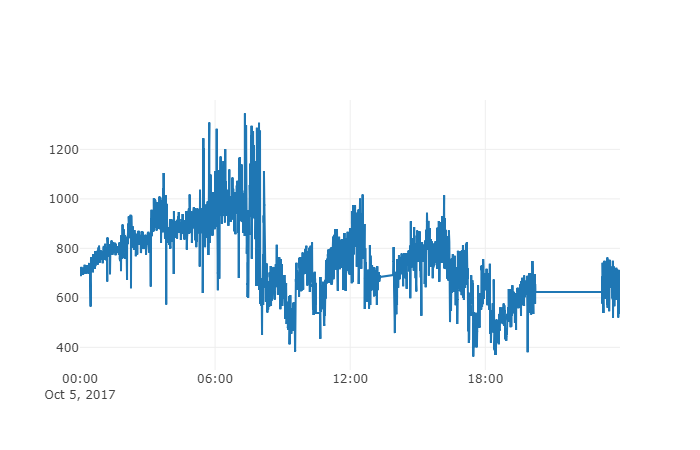
\includegraphics[width=0.7\textwidth]{raw_day}
            	\caption{Série temporal dos intervalos R-R registrados durante um dia. A série foi suavizada com uma média móvel de meia-janela de 15 pontos para facilitar a visualização. Os intervalos são mais espaçados e irregulares em situações de relaxamento como o sono, e mais curtos e regulares durante o movimento ou em situações de estresse}
                \label{raw_day}
            \end{figure}
        
        \subsection{Remoção de outliers e artefatos}
        
            \paragraph{} Apesar do posicionamento do coração garantir um sinal mais limpo do que o de EEG, esse sinal não é, naturalmente, livre de ruídos e artefatos. Uma causa natural para a geração de ruído são os batimentos ectópicos, que são causados por condução elétrica originada em fibras fora do nó sinoatrial (sinoatrial node), região do músculo cardíaco responsável pelos impulsos elétricos que causam os batimentos regulares. Além disso, há a possibilidade de mal funcionamento no hardware do sensor, seja por falta de contato com a pele para detectar o impulso ou por falha no algoritmo interno de detecção do complexo QRS. 
            
            \paragraph{} Para remover esse tipo de ruído, aplicamos no dado um filtro para remoção de outliers que consiste em duas estratégias. A primeira é remover todos os intervalos com valores absolutos fora de um \textit{threshold}, que é configurável na execução do pipeline. Para as análises apresentadas nesse trabalho, consideramos aceitáveis os intervalos dentro do limite $300 <= RR <= 1800$. 
            
            \paragraph{} A segunda estratégia é baseada em uma média móvel que nos permite definir se um intervalo é um \textit{outlier} relativo ao contexto em que se encontra. Definimos como uma \textbf{sequência contínua} qualquer sequência de intervalos R-R que não tenha um \textit{gap} maior que 3s entre seus \textit{timestamps}. Sempre que ocorre um \textit{gap} maior que esse valor entre dois intervalos consecutivos nos dados, uma sequência é quebrada no primeiro e outra iniciada no segundo intervalo. Para cada uma dessas sequências, passamos um filtro de média-móvel com meia-janela de tamanho 10 intervalos (total de 21 na janela) e, quando um intervalo está mais de 3 desvios-padrão acima ou abaixo da janela centrada nele próprio, ele é considerado um \textit{outlier} e removido.

            %%JUINCLUDEFIGURE comparação de um dado com e sem outlier/ectopic beat
        
        \subsection{Extração de sessões}
        
            \paragraph{} Até esse ponto, o pipeline trabalha com todos os intervalos disponíveis. Todavia, nem todos são usados na classificação de atividades, visto que o aplicativo permanece coletando-os enquanto o sensor estiver ativo, mesmo fora do tempo das atividades registradas pelo indivíduo. O próximo passo do pipeline é, portanto, extrair do banco de dados de intervalos apenas os que fazem parte de alguma atividade e agrupá-los com as informações das atividades registradas. Definimos esse conjunto de dados como \textbf{sessão}. Uma sessão é constituída por:
            
            \begin{itemize}
                \item O tipo da atividade exercida;
                \item O horário de início da sessão, para referência posterior;
                \item A duração total, calculada pelo final da atividade informada pelo indivíduo. Não necessariamente os intervalos registrados cobrem todo o período. É possível, por exemplo, que o sensor perca contato com o aparelho de celular com o qual estava conectado, interrompendo a sequência de intervalos antes do fim da atividade.
                \item Todos os intervalos do banco que estejam contidos no período entre o início e o fim da atividade;
            \end{itemize} 
            
            \paragraph{} A seleção dos intervalos que estão contidos em uma sessão é determinada pelo \textit{timestamp} dos eventos. Cabe ressaltar que o sensor apenas provê o valor em ms do intervalo, não contando com um \textit{timestamp}, que é adicionado no aplicativo de coleta, com frequência de 1Hz. Dessa forma, a referência que consta no intervalo armazenado no banco de dados é ao momento em que o intervalo foi recebido e não do batimento. No entanto, como nossa análise é realizada sobre o comprimento dos intervalos e suas relações com intervalos consecutivos, isso não afeta nossa medição.
            
            %%JUINCLUDEFIGURE visualização de dois ou três tipos de sessão (histograma/time series)
            
            
        \subsection{Fragmentação} \label{fragdesc}
        
            \paragraph{} Conforme recomendações para a análise de HRV \cite{Quintana2016GuidelinesCommunication}, optamos por fragmentar cada sessão em segmentos de igual duração para que possam ser comparados dentro dos mesmos parâmetros. Caso contrário, haveria um desequilíbrio entre sessões de atividades cuja duração é muito diferente, por exemplo, uma sessão de sono de 8h e uma sessão de corrida de 15 minutos. Em geral \cite{TaskForceoftheEuropeanSocietyofCardiologytheNorthAmericanSocietyofPacing1996HeartUse, Shaffer2017AnNorms.}, a análise de HRV é descrita como sendo de curta duração se tiver em torno de 5 minutos, e de ultra-curta duração se tiver menos tempo.
            
            \paragraph{} O pipeline implementado permite a configuração da duração de cada fragmento. Além disso, é possível também configurar um período chamado de \textit{crop}, que é removido do início de cada sessão e não entra nos fragmentos, para suprimir o possível ruído causado pela adaptação da frequência cardíaca do indivíduo ao início da nova tarefa. Com esses dos parâmetros, são gerados o tempo de início e fim de cada fragmento dentro de uma sessão. Assim como na geração da sessão, os intervalos contidos em cada fragmento são determinados através da comparação de seu \textit{timestamp} com os horários de início e fim determinados para o fragmento. 
            
        \subsection{Cálculo das métricas agregadas}
        
            \paragraph{}A seguir, são calculadas as métricas agregadas da distribuição dos intervalos, conforme descritas na seção ~\ref{HRV}. Calculamos essas métricas para a distribuição dos intervalos tanto das sessões como dos fragmentos. Apesar de apenas os fragmentos serem utilizados na análise de dados e nos classificadores, as métricas das sessões são úteis para análise exploratória, visualização e comparação das sessões por tipo de atividade. As métricas utilizadas são descritas na tabela ~\ref{feats}:
  
            \begin{table}[h!]
                \centering
                \begin{tabular}{ll}
                MRRI  & média dos valores dos intervalos                             \\
                SDNN  & desvio-padrão dos valores dos intervalos                     \\
                RMSSD & média RMS dos valores das diferenças entre dois intervalos consecutivos \\
                PNN50 & porcentagem dos intervalos consecutivos cuja diferença é superior a 50ms \\
                LFNU  & valor normalizado da potência do espectro na faixa 0.04–0.15Hz\\
                HFNU  & valor normalizado da potência do espectro na faixa 0.15–0.40Hz\\
                HF:LF & razão entre os valores de hf e lf
                \end{tabular}
                \caption{Métricas agregadas calculadas para cada fragmento e sessão e utilizadas na análise dos dados e classificação}
                \label{feats}
            \end{table}
            
            \paragraph{}Apesar de armazenados, valores como MHR (média de frequência cardíaca) e NN50 (número absoluto de intervalos consecutivos cuja diferença é superior a 50ms), LF e HF (valores absolutos da potência do espectro na baixa e alta frequências, em ms\textsuperscript{2}) não são utilizados nas análises, por serem diretamente correlacionados, respectivamente com o MRRI, PNN50, LFNU e HFNU, das quais derivam ou são derivados diretamente, sendo, portanto, redundantes. Além disso, a VLF (potência do espectro na faixa de 0.0003Hz a 0.04Hz) também é armazenada, mas não utilizada nas análises porque seu período (25s a 333s) elevado inviabiliza a presença de ciclos suficientes em dados de ultra-curta duração.
        
           \paragraph{} Cada execução completa do pipeline, desde a remoção de artefatos até o cálculo das métricas, leva à geração de um \textit{dataset} para análise. Para a geração desse \textit{dataset} são excluídas as listas de intervalos e mantidas apenas as métricas agregadas e dados do fragmento e de sua sessão relacionada. Cada linha, portanto, tem o seguinte conteúdo:
                \begin{itemize}
                    \item id do usuário;
                    \item descrição da atividade;
                    \item índice identificador da sessão;
                    \item índice da ordenação relativa do fragmento dentro da sessão (esse dado nos permite, por exemplo, normalizar análises usando apenas os n primeiros fragmentos de cada sessão);
                    \item \textit{timestamp} do início do fragmento;
                    \item todas as métricas agregadas descritas acima, incluindo as que não são usadas nas análises mas podem ser visualizadas, num total de 12 métricas.
                \end{itemize}
                
            \paragraph{} A nomenclatura do \textit{dataset} gerado indica os parâmetros escolhidos para \textit{crop} e duração. No intuito de definir a configuração ótima deses parâmetros, executamos o pipeline repetidamente, variando os valores desses dois parâmetros gernado um \textit{dataset} para cada par de parâmetros. Os valores testados foram (em segundos): 30, 60, 90 para o \textit{crop} e 60, 120, 180, 240, 300, 420, 600 para a duração.
        
            %%JUINCLUDEFIGURE exemplo de fragmento
            %%JUINCLUDEFIGURE diagrama do pipeline
        
%----------------------------------------------------------------------------------------
%	CLASSIFICATION
%----------------------------------------------------------------------------------------
        
        
    \section{Classificação supervisionada de atividades}
    \label{Activities}

        \subsection{Feature engineering}
        
            \subsubsection{Comprimento dos fragmentos}
            
            \subsubsection{Controle de ruído vs overfitting}
            
            \subsubsection{Controle de outliers}
    
        \subsection{SVM x Random Forest}
        
        \subsection{Hierarquia}
        
        
\chapter{Discussão}
\label{Dicussion}